\documentclass{scrartcl}

\usepackage[utf8]{inputenc}
\usepackage[T1]{fontenc}
\usepackage{lmodern}
\usepackage[english]{babel}
\usepackage{amsmath}
\usepackage{graphicx}
\usepackage{caption}	
\usepackage{subcaption}	 
\usepackage{hyperref}
\usepackage[parfill]{parskip}
\usepackage{hhline}

\title{Neuroprosthetics - Exercise 2}
\author{Alexander Koenig}
\date{24. November 2019}

\begin{document}
\maketitle

\section{Plot Slope Fields and Isoclines}

Figures \ref{fig:ode1} and \ref{fig:ode2} show the slope fields and isoclines for the ordinary differential equations (ODE) 1 and 2 respectively. An isocline is a line at which the slope (here $\frac{dV}{dt}$) equals to a constant $k$. The isoclines for the set of constants $K = \{-2, -1, 0, 1, 2\}$ are plotted.

\begin{equation}
	\label{eq:ode_1}
	\frac{dV}{dt} = 1 - V - t  
\end{equation}
\begin{equation}
	\label{eq:ode_2}
	\frac{dV}{dt} = sin(t) - \frac{1}{1.5}V 
\end{equation}

\begin{figure}[h]
	\centering
	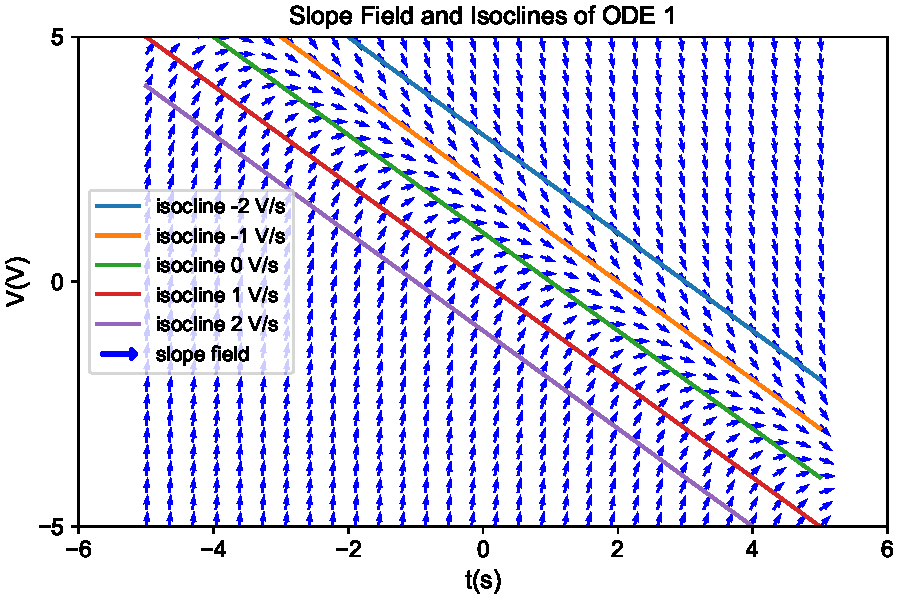
\includegraphics[width=0.9\textwidth]{figures/ode_1.pdf}
	\caption{Slope field and isoclines of ODE 1}
	\label{fig:ode1}
\end{figure}

\newpage
\begin{figure}[h]
	\centering
	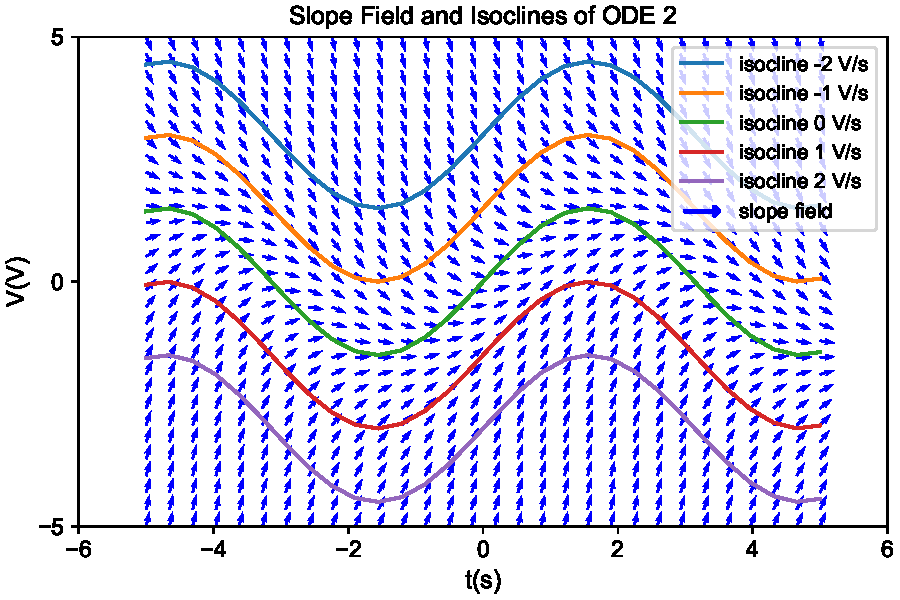
\includegraphics[width=0.9\textwidth]{figures/ode_2.pdf}
	\caption{Slope field and isoclines of ODE 2}
	\label{fig:ode2}
\end{figure}

\newpage

\section{Differential Equations of a Simple Cell Model}

The differential equation of the leaky integrate and fire neuron model can be derived from Kirchhoffs law as shown in equation \ref{eq:kirchhoff}. The external current is known and defined by equation \ref{eq:iex}. The expression for the current through the resistor $I_{r}$ in equation \ref{eq:ir} can simply be derived from Ohm's law $R = \frac{V}{I}$. Furthermore, the capacitor's displacement current in equation \ref{eq:ic} can be derived from the relations $I = \frac{dQ}{dt}$ and $Q = C \cdot V$. 

\begin{equation}
	\label{eq:kirchhoff}
	I_{ex}(t) = I_{r}(t) + I_{c}(t)
\end{equation}
\begin{equation}
	\label{eq:iex}
	I_{ex}(t) = I_{max} \cdot sin(t) 
\end{equation}
\begin{equation}
	\label{eq:ir}
	I_{r}(t) = \frac{V_{r}(t)}{R_{l}}  
\end{equation}
\begin{equation}
	\label{eq:ic}
	I_{c}(t) = C_{m} \cdot \frac{dV}{dt}  
\end{equation}

By plugging the results for the components' currents in the original formula \ref{eq:kirchhoff} we get equation \ref{eq:res} and by rearranging we obtain the final governing differential equation \ref{eq:end}. The exercise asks to include another constant term $D$ to the current part of the differential equation, which is done in equation \ref{eq:endD}.

\begin{equation}
	\label{eq:res}
	I_{max} \cdot sin(t) = \frac{V_{r}(t)}{R_{l}} + C_{m} \cdot \frac{dV}{dt}
\end{equation}
\begin{equation}
	\label{eq:end}
	\frac{dV}{dt} = \frac{1}{C_{m}}\bigg( I_{max}\cdot sin(t) - \frac{V_{r}(t)}{R_{l}}\bigg)
\end{equation}
\begin{equation}
	\label{eq:endD}
	\frac{dV}{dt} = \frac{1}{C_{m}}\bigg( I_{max}\cdot sin(t) + D - \frac{V_{r}(t)}{R_{l}}\bigg)
\end{equation}

Finally, plots of this ordinary differential equation are presented. There are four plots with the following parameters.


\begin{table}[h]
\vspace{0.5cm}
\centering
\begin{tabular}{|l|l|l|l|l|}
\hline
$R$                      & $C_{m}$ & $I_{max}$ & $D$ & Plot \\ \hhline{|=|=|=|=|=|}

1.3$\Omega$ & 0.8F    & 0A        & 0A  & A    \\ \hline
1.3$\Omega$ & 0.8F    & 1A        & 0A  & B    \\ \hline
1.3$\Omega$ & 0.8F    & 0A        & 2A  & C    \\ \hline
1.3$\Omega$ & 0.8F    & 1A        & 2A  & D    \\ \hline
\end{tabular}
\label{tab:values}
\end{table}

\begin{figure}[h]
	\centering
	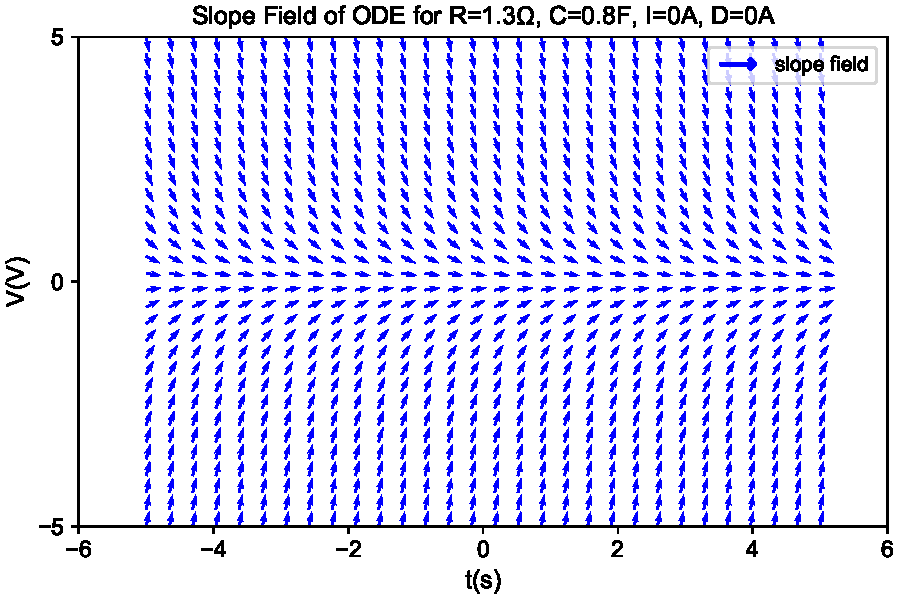
\includegraphics[width=0.9\textwidth]{figures/ode_3_i0_d0.pdf}
	\caption{Plot A}
\end{figure}

\begin{figure}[h]
	\centering
	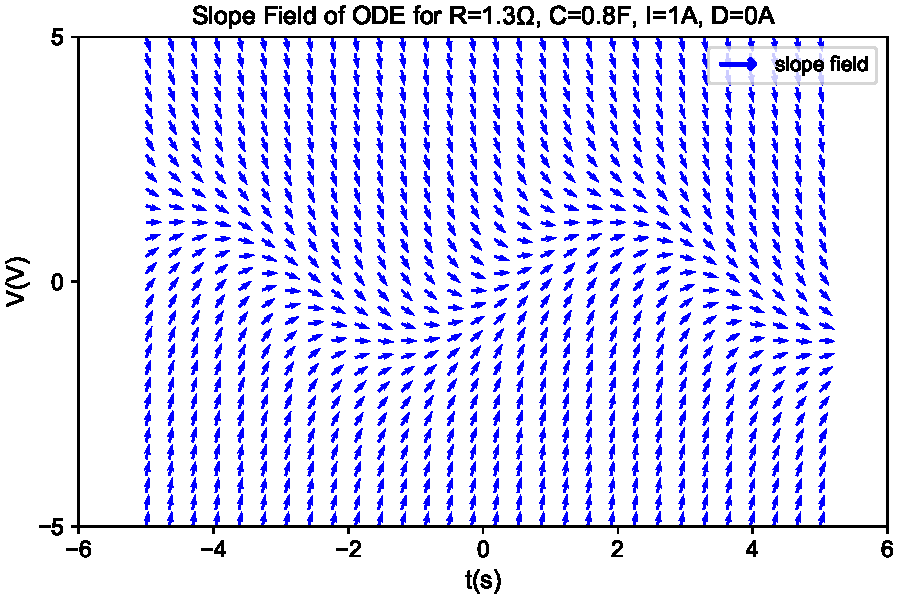
\includegraphics[width=0.9\textwidth]{figures/ode_3_i1_d0.pdf}
	\caption{Plot B}
\end{figure}

\begin{figure}[h]
	\centering
	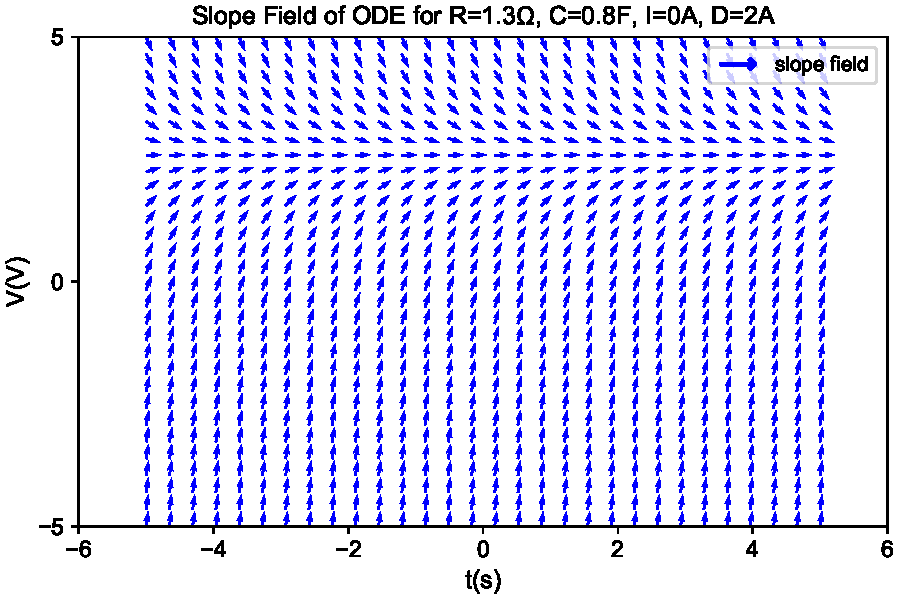
\includegraphics[width=0.9\textwidth]{figures/ode_3_i0_d2.pdf}
	\caption{Plot C}
\end{figure}

\begin{figure}[h]
	\centering
	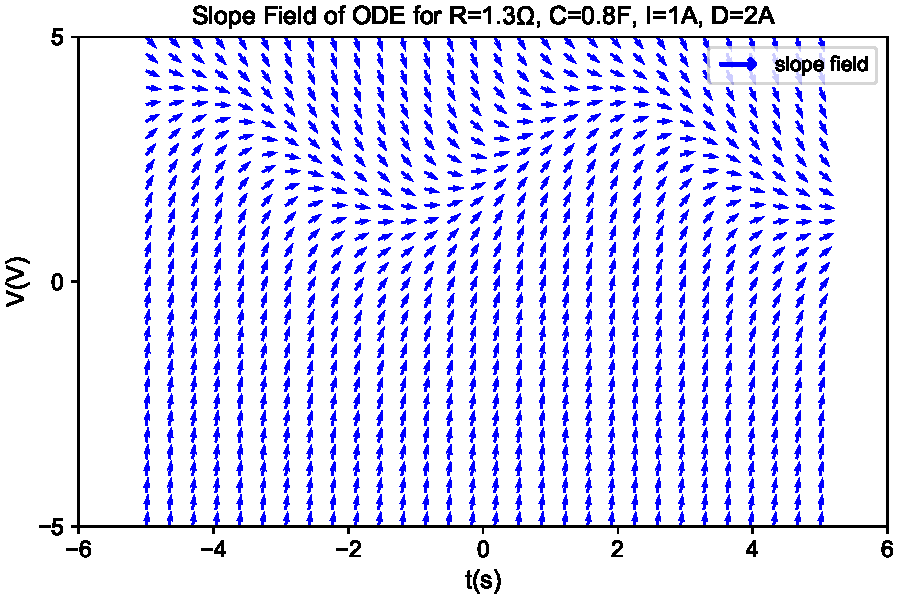
\includegraphics[width=0.9\textwidth]{figures/ode_3_i1_d2.pdf}
	\caption{Plot D}
\end{figure}


\end{document}